\section{Introduction and project objectives}
Cooling and heating equipment depends on sensors to regulate temperature, airflow and pressure. A biased sensor can report a plausible value while the control system responds to an incorrect representation of the unit. Detecting the abnormal condition is useful, but identifying which sensor is affected provides a more specific diagnostic output. This project studies that problem with a Long Short-Term Memory (LSTM) network using short histories of operating measurements.

The project progressed through two distinct tasks. The earlier model detected outdoor-air temperature sensor bias in a simulated air-handling unit (AHU). It already accepted several measurement and control channels, but its output remained binary: healthy or outdoor-air sensor fault. The extension changes the output to five conditions: healthy operation and four individual sensor faults at cold-deck and hot-deck temperature and pressure locations. Outdoor-air temperature bias is not one of these four new targets.

The extension uses a separate dual-duct simulation dataset, different fault definitions and a different calendar partition. It therefore demonstrates broader diagnostic scope within that simulation; a comparison of the two headline accuracies cannot establish a matched improvement. The central deep learning contribution is the complete sequence-classification pipeline: explicit data eligibility, training-only transformations, a compact LSTM, input-reduction experiments, validation-based checkpoint and alarm selection, and evaluation on reserved calendar periods.

The objectives are to identify the correct faulty sensor, compare all 26 declared inputs with five training-selected inputs, and quantify false alarms during healthy operation. The validation gate requires healthy false-positive rate (FPR) at or below 1\% and correct-sensor recall of at least 40\% for every fault class. Five-class accuracy and macro F1 complement these constraints. The final evaluation must retain failures against the original goal rather than reinterpret the goal after observing test results.

The resulting prototype achieves 92.87\% five-class test accuracy and 89.36\% macro F1. Its healthy FPR is 2.10\%, so the reserved test does not meet the 1\% target. The report explains both the useful diagnostic performance and this unresolved limitation. It covers one simulated unit with one imposed sensor bias per scenario; it does not establish field deployment reliability or future-failure forecasting.

\section{Background and the role of temporal learning}
\subsection{Detection, diagnosis and the observation window}
A detection task asks whether a fault is present. A diagnostic task additionally assigns a fault type. In the four-sensor study, a pressure fault labeled as a temperature fault is still a diagnostic error, even though an alarm was raised. Healthy false alarms, missed faults and wrong-sensor alarms consequently require separate accounting.

An individual sensor reading may be insufficient to distinguish bias from a normal operating transition. A sequence includes how temperatures, fan speeds, airflow and commands evolve together. The project uses the current minute and 29 preceding minutes, giving a 30-step input. This is retrospective classification at the current endpoint. No future reading is supplied, and the experiment is not a forecast of a fault that has yet to occur.

\subsection{LSTM memory and gates}
An LSTM maintains cell and hidden states to control information retained from a sequence~\cite{hochreiter1997}. The following gates follow the modern PyTorch implementation, including its forget gate~\cite{pytorch}. For input $\mathbf{x}_t$, previous hidden state $\mathbf{h}_{t-1}$ and cell state $\mathbf{c}_{t-1}$,
\begin{align}
\mathbf{i}_t &= \sigma(W_i\mathbf{x}_t+U_i\mathbf{h}_{t-1}+\mathbf{b}_i), &
\mathbf{f}_t &= \sigma(W_f\mathbf{x}_t+U_f\mathbf{h}_{t-1}+\mathbf{b}_f),\\
\mathbf{g}_t &= \tanh(W_g\mathbf{x}_t+U_g\mathbf{h}_{t-1}+\mathbf{b}_g), &
\mathbf{o}_t &= \sigma(W_o\mathbf{x}_t+U_o\mathbf{h}_{t-1}+\mathbf{b}_o),\\
\mathbf{c}_t &= \mathbf{f}_t\odot\mathbf{c}_{t-1}+\mathbf{i}_t\odot\mathbf{g}_t, &
\mathbf{h}_t &= \mathbf{o}_t\odot\tanh(\mathbf{c}_t).
\end{align}
Here $\sigma$ is the sigmoid function and $\odot$ denotes elementwise multiplication. The forget gate controls retained memory; the input gate controls new content; and the output gate controls the exposed hidden representation. The final hidden state summarizes the 30 readings for the classifier. States are not carried between independently scored windows.

The architecture is deliberately small enough for saved-model CPU inference. Using an LSTM does not by itself prevent leakage or guarantee low false alarms. Calendar separation, causal cleaning and explicit operating eligibility are as important as the neural layer when assessing whether the reported performance is credible.

\section{Datasets and the expansion of diagnostic scope}
\subsection{Earlier outdoor-air temperature detector}
The earlier benchmark uses the original \texttt{MZVAV-1.csv} file from the LBNL AFDD collection, DOI \url{https://doi.org/10.25984/1824861}. It contains 272,160 one-minute readings across 189 source days. Native labels identify normal operation and outdoor-air temperature sensor biases of $\pm1$, $\pm2$ and $\pm4\,^{\circ}\mathrm{C}$. The measurement columns retain Fahrenheit units. These are simulated AHU measurements, not observations of a datacenter cooling failure.

Winter and spring form training, summer forms validation, and autumn forms the reserved test. Entire source days and scenario blocks remain in one partition. Thirteen raw inputs, six consistency features and thirteen missing indicators produce 32 model channels. The consistency features include temperature differences and a command-weighted mixing residual; the latter is a proxy rather than a measurement of mixing airflow fraction.

\begin{table}[htbp]\centering\small
\caption{Partition sizes for the earlier outdoor-air detector.}\label{tab:old-split}
\begin{tabularx}{\linewidth}{l X r r}
\toprule
Partition & Seasons & Raw/scored days & Scored endpoints \\
\midrule
Train & Winter and spring & 91/77 & 61,187 \\
Validation & Summer & 49/42 & 33,432 \\
Test & Autumn & 49/42 & 33,432 \\
\bottomrule\end{tabularx}
\end{table}

The predeclared primary seed is 42. Its frozen two-of-three alarm rule gives 92.82\% autumn accuracy, 99.74\% alarm precision, 91.86\% fault-reading recall and 1.44\% FPR. The confusion counts are TP 26,324, FP 69, FN 2,332 and TN 4,707. The false readings form one burst. These results motivate reporting false alarms explicitly: high precision does not imply that the original 1\% FPR target was satisfied. The earlier experiment remains available separately in the dashboard and code bundle.

\subsection{Dual-duct source for four-sensor diagnosis}
The extension uses the public LBNL simulated dual-duct AHU source~\cite{lbnl2022,granderson2023}. A dual-duct unit provides cold and hot air streams, allowing the experiment to label temperature and duct-pressure sensor biases at both supply decks. The source archive contains 56 CSV files and 114 recorded measurement or control points. Seventeen native scenarios are selected: one healthy case and sixteen biased cases, representing four source severity identifiers at each of four sensor locations.

Each selected file contains 525,600 one-minute rows from 2018. The resulting 8,935,200 source rows represent parallel scenarios of one modeled system, rather than seventeen independently operated units. The source authors supply the scenario labels. Timestamp, scenario identifier, filename severity and class labels are excluded from the neural input.

Source integrity is checked before learning. An initially considered single-duct download was rejected because four outdoor-air bias tables were identical and the documented supply-air bias filenames were absent. Its audit is retained, and those cases do not enter this extension. The accepted dual-duct cases have distinct archive signatures and traces.

The pressure filenames contain native $\pm2$ and $\pm4$ \texttt{inwg} identifiers, whereas Table 4 of the source paper documents $\pm0.2$ and $\pm0.4\,\mathrm{inH_2O}$. The project retains original identifiers and does not claim independently verified pressure offset magnitudes. Temperature measurements remain in Fahrenheit. Maintaining this distinction avoids silently converting a filename into an unsupported physical-severity claim.

\begin{table}[htbp]\centering\small
\caption{Output classes in the four-sensor extension.}\label{tab:classes}
\begin{tabularx}{\linewidth}{c l X}
\toprule
Code & Condition & Diagnostic interpretation \\
\midrule
H & Healthy & No modeled sensor bias \\
CT & Cold-deck temperature & Bias at the cold supply-air temperature sensor \\
HT & Hot-deck temperature & Bias at the hot supply-air temperature sensor \\
CP & Cold-deck pressure & Bias at the cold supply-duct pressure sensor \\
HP & Hot-deck pressure & Bias at the hot supply-duct pressure sensor \\
\bottomrule\end{tabularx}
\end{table}

\section{Experimental protocol and preprocessing}
\subsection{Calendar separation across parallel scenarios}
Randomly splitting overlapping minute windows could place the same operating period into both training and evaluation. The extension instead assigns whole ISO calendar weeks with a fixed rule. If week number $w$ satisfies $w\bmod6=0$, its readings belong to test; if $w\bmod6=5$, they belong to validation; all other weeks belong to training. Every scenario uses the same assignment. Matching weather and operating periods therefore remain together across the seventeen parallel files.

This design evaluates held-out periods of the same simulated unit and known fault families. It does not test transfer to a new physical AHU or unseen fault severity. Training, checkpoint selection and policy selection also use different endpoint sampling rates, as shown in Table~\ref{tab:new-split}. The millions of eligible endpoints must not be described as the number of independent optimized training examples.

\begin{table}[htbp]\centering\small
\caption{Eligible endpoints and optimization sampling in the extension.}\label{tab:new-split}
\begin{tabularx}{\linewidth}{l r X}
\toprule
Partition & Eligible endpoints & Use in the experiment \\
\midrule
Training & 2,096,259 & 36,404 hourly endpoints for optimization \\
Validation & 463,842 & 30,877 quarter-hour endpoints for checkpoints; every eligible minute for policies \\
Reserved test & 463,058 & Every eligible minute after the model and policy were frozen \\
\bottomrule\end{tabularx}
\end{table}

\subsection{Operating eligibility and sequence construction}
A scored endpoint requires 30 consecutive one-minute readings within one scenario and one source day. All readings must satisfy \texttt{SYS\_CTL=1}, with both cold and hot supply fan speeds positive. Windows reset at day, scenario and cadence boundaries; a history cannot bridge a shutdown or a missing interval. Inactive periods remain outside the scored task, and raw versus scored day counts are retained to make that coverage restriction visible.

For a valid endpoint $t$, the transformed input is
\begin{equation}
X_t=[\mathbf{z}_{t-29},\ldots,\mathbf{z}_{t}]\in\mathbb{R}^{30\times d},
\end{equation}
where $d=26$ for the full model and $d=5$ for the input-reduction experiment. The endpoint class is the original scenario label. Overlapping windows contain repeated information; the test row count is an amount of scored time, not a count of independent units.

\subsection{Causal cleaning and training-only statistics}
The pipeline keeps valid negative outdoor temperatures in Fahrenheit. Nonfinite values receive at most five causal forward-filled readings within a continuous day segment. It never uses a later observation to fill an earlier gap. Remaining gaps use per-channel medians estimated from healthy, active training rows. Mean and standard deviation are also fitted on those training rows; channels with effectively zero scale use a scale of one. The transformation is
\begin{equation}
z_{t,j}=\operatorname{clip}\!\left(\frac{\widetilde{x}_{t,j}-\mu_j}{s_j},-10,10\right),
\end{equation}
where $\widetilde{x}_{t,j}$ is the causally completed value. The saved training statistics are reused unchanged for validation, test and uploaded CSVs. No nonfinite values appeared in the audited training columns, but retaining a deterministic missing-value rule keeps the inference interface explicit. It does not establish robustness to arbitrary sensor dropouts.

\begin{table}[htbp]\centering\small
\caption{Declared full-model input groups.}\label{tab:inputs}
\begin{tabularx}{\linewidth}{X r X}
\toprule
Input group & Count & Examples or scope \\
\midrule
Air temperatures & 5 & Cold supply, hot supply, outdoor, mixed and return air \\
Duct pressures & 2 & Cold and hot supply pressure \\
Humidity measurements & 4 & Outdoor, return, cold supply and hot supply \\
Airflow measurements & 4 & Cold supply, hot supply, outdoor and return airflow \\
Fan speed measurements & 3 & Cold supply, hot supply and return fan speed \\
Fan power measurements & 3 & Cold supply, hot supply and return fan power \\
Control commands & 5 & Outdoor, return and exhaust dampers; chilled-water and hot-water valves \\
\bottomrule\end{tabularx}
\par\smallskip\footnotesize The 26 inputs comprise 21 measurements and five commands. The operating-control flag is used for eligibility, not as a neural feature.
\end{table}

\begin{figure}[htbp]
\centering
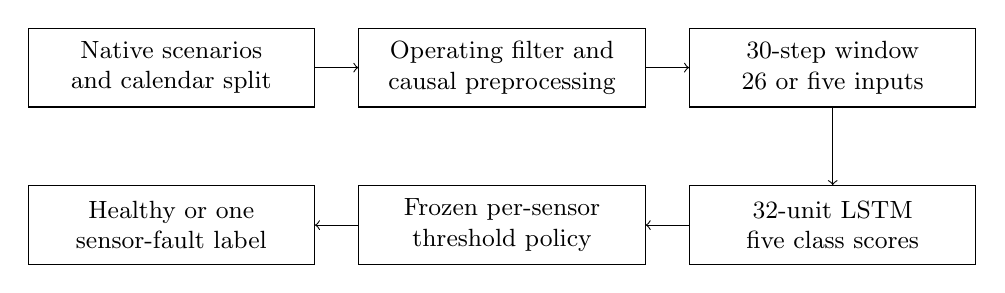
\begin{tikzpicture}[every node/.style={font=\small,align=center}]
\node[draw,text width=3.4cm,minimum height=1.0cm] (a) at (0,2.0) {Native scenarios\\and calendar split};
\node[draw,text width=3.4cm,minimum height=1.0cm] (b) at (4.2,2.0) {Operating filter and\\causal preprocessing};
\node[draw,text width=3.4cm,minimum height=1.0cm] (c) at (8.4,2.0) {30-step window\\26 or five inputs};
\node[draw,text width=3.4cm,minimum height=1.0cm] (d) at (8.4,0) {32-unit LSTM\\five class scores};
\node[draw,text width=3.4cm,minimum height=1.0cm] (e) at (4.2,0) {Frozen per-sensor\\threshold policy};
\node[draw,text width=3.4cm,minimum height=1.0cm] (f) at (0,0) {Healthy or one\\sensor-fault label};
\draw[->] (a)--(b);\draw[->] (b)--(c);\draw[->] (c)--(d);\draw[->] (d)--(e);\draw[->] (e)--(f);
\end{tikzpicture}
\caption{End-to-end sequence diagnosis. Preprocessing statistics are fitted on healthy training rows; checkpoints and alarm policies use validation only.}
\label{fig:pipeline}
\end{figure}

\section{Deep learning architecture and training}
\subsection{Compact multiclass LSTM}
The network contains one 32-unit LSTM layer, followed by a 16-unit fully connected layer, ReLU activation, dropout with probability 0.2, and five output logits. The head reads the last hidden state. Softmax converts logits into normalized class scores for inference, but the scores have not been probability calibrated.

For the full-input model, the implementation has 8,293 trainable parameters. With PyTorch's separate input and recurrent bias vectors, the count is
\begin{equation}
4h(d+h+2)+(h\cdot16+16)+(16\cdot5+5)=8,293,
\end{equation}
where $h=32$ and $d=26$. Reducing $d$ to five gives 5,605 parameters while retaining the same hidden layer and classifier head. The reduced experiment therefore changes the information supplied to the network rather than introducing a different family of neural architecture.

\subsection{Weighted loss and optimization}
Training uses weighted multiclass cross entropy and Adam with learning rate 0.001~\cite{kingma2015}. Batch size is 512, and the gradient norm is clipped to one. For labels $y_n$, class scores $p_{n,k}$ and class weights $\alpha_k$, the batch objective is
\begin{equation}
\mathcal{L}=-\frac{\sum_n\alpha_{y_n}\log p_{n,y_n}}{\sum_n\alpha_{y_n}}.
\end{equation}
Version 1 uses inverse-frequency weights $N/(5N_k)$. Version 2 doubles the healthy-class weight while retaining the other class weights. The healthy optimization class contains 2,172 windows, compared with 8,168 cold-temperature and 8,688 windows for each remaining fault class. Doubling healthy weight gives this underrepresented condition more influence on the loss without changing evaluation prevalence.

The primary seed is fixed at 42 for Python, NumPy, PyTorch and the shuffled training loader. The extension does not report repeated-seed robustness. Saving a deterministic run improves reproducibility, but it does not measure the distribution of outcomes under other initializations.

\subsection{Logged development versions and checkpoint choice}
Version 1 trains the 26-input and five-input LSTMs for at most 20 epochs, with four-epoch patience. Its checkpoint criterion is mean average precision across the four fault classes. Neither family satisfies the combined healthy-FPR and each-sensor-recall validation gate.

Version 2 records a validation refinement before opening the reserved test. It increases the budget to 80 epochs with eight-epoch patience, doubles the healthy loss weight and selects checkpoints by macro average precision across all five classes, including healthy. The five-input ranking is reused rather than reranked. Four unique networks are trained across the two versions; Version 2 also evaluates the two retained Version 1 networks under its expanded policy search.

The selected full-input Version 2 run stops after 50 epochs and restores epoch 42. Its checkpoint validation macro average precision is 0.9969. Figure~\ref{fig:learning} plots its saved training loss and checkpoint-validation metric. The learning curves describe optimization and checkpoint selection; they do not substitute for the reserved test or justify further tuning after the test has been inspected.

\begin{figure}[htbp]\centering
\begin{minipage}{0.48\linewidth}\centering
\begin{tikzpicture}
\begin{axis}[width=0.96\linewidth,height=5.1cm,xlabel={Epoch},ylabel={Training loss},xmin=1,xmax=50,grid=major,tick label style={font=\footnotesize},label style={font=\small}]
\addplot[thick] table[x=epoch,y=train_loss,col sep=comma]{data/training_history.csv};
\end{axis}\end{tikzpicture}
\end{minipage}\hfill
\begin{minipage}{0.48\linewidth}\centering
\begin{tikzpicture}
\begin{axis}[width=0.96\linewidth,height=5.1cm,xlabel={Epoch},ylabel={Validation macro AP},xmin=1,xmax=50,ymin=0.3,ymax=1.02,grid=major,tick label style={font=\footnotesize},label style={font=\small}]
\addplot[thick] table[x=epoch,y=validation_macro_ap_all_classes,col sep=comma]{data/training_history.csv};
\addplot[dashed] coordinates {(42,0.3)(42,1.02)};
\end{axis}\end{tikzpicture}
\end{minipage}
\caption{Editable plots from the saved full-input Version 2 history. The dashed line marks the restored checkpoint at epoch 42.}
\label{fig:learning}\end{figure}

\section{Training-only feature selection and input ablation}
The five-input comparison tests whether a much smaller set of raw channels retains enough information for fault identification. A separate Extra Trees selector receives four summaries per candidate channel: latest value, mean, standard deviation and slope over the same history. It fits an internal subset of training weeks and measures balanced log-loss changes on held-out training weeks. The selector is a ranking tool; the submitted classifier remains an LSTM.

Permutation moves complete daily trajectories, jointly across a channel's four summaries, with three fixed repeats. Validation and test labels do not enter the ranking. This grouping reduces the distortion that would result from independently shuffling adjacent minute observations. Correlated measurements can still share predictive information, so the ranking is conditional on the selector and its internal split. It is not an exhaustive search for the globally best subset.

\begin{table}[htbp]\centering\small
\caption{Five selected raw inputs, in training-only importance order.}\label{tab:five}
\begin{tabularx}{\linewidth}{l X l}
\toprule
Source alias & Meaning & Input type \\
\midrule
\texttt{HSF\_SPD} & Hot supply fan speed & Measurement \\
\texttt{HSF\_WAT} & Hot supply fan power & Measurement \\
\texttt{CSF\_SPD} & Cold supply fan speed & Measurement \\
\texttt{CHWC\_VLV\_DM} & Chilled-water valve command & Command \\
\texttt{CSF\_WAT} & Cold supply fan power & Measurement \\
\bottomrule\end{tabularx}
\end{table}

The selected set contains four measurements and one command. It is not the set of four fault-target sensors plus one extra sensor. Both five-input LSTMs fail validation targets and perform substantially worse on the reserved test. Removing direct temperatures and pressures can remove relationships useful for sensor localization, even when a tree assigns high conditional importance to fan and valve channels. This evidence supports retaining the 26-input model for this study. It does not establish that every engineered five-feature model would fail. Principal component analysis is not implemented in the submitted experiment.

\section{Alarm policy and evaluation measures}
\subsection{Converting class scores into a diagnostic output}
A raw softmax argmax is not the final alarm rule. Each fault class $k\in\{1,2,3,4\}$ has a validation-derived threshold $\tau_k$. Candidate rules require an immediate threshold crossing, two consecutive crossings, or two crossings in three consecutive scored minutes. Persistence state resets at day, scenario and gap boundaries. When multiple fault classes qualify, the policy selects the highest eligible class score; when none qualifies, it returns healthy.

Version 2 compares 126 policies for each of four candidates, totaling 504 final validation policies. The search includes shared healthy-score percentiles and configurations allocating a larger false-alarm budget to one fault class. The earlier Version 1 policy search is also retained in the development record. Validation macro F1 selects among candidates satisfying FPR $\leq1\%$ and every fault-class recall $\geq40\%$. Model, transformations and policy are frozen before one-time test inference.

The selected rule is immediate, with thresholds 0.928234, 0.982397, 0.585455 and 0.908126 for CT, HT, CP and HP respectively. A score exceeding its class threshold can therefore raise an alarm at the current endpoint. These values are frozen decision thresholds, not calibrated confidence guarantees.

\subsection{Metrics and their denominators}
For each class, precision is $TP/(TP+FP)$, recall is $TP/(TP+FN)$, and F1 is their harmonic mean. Macro F1 averages the five class F1 scores equally. Accuracy counts only predictions with the correct complete class label. Any-fault detection recall instead counts a fault as detected whenever the output is any nonhealthy class, including a wrong-sensor alarm.
\begin{equation}
\mathrm{Healthy\ FPR}=\frac{\#\{y=0,\widehat{y}\ne0\}}{\#\{y=0\}},\qquad
\mathrm{Fault\ recall}=\frac{\#\{y\ne0,\widehat{y}\ne0\}}{\#\{y\ne0\}}.
\end{equation}
Healthy FPR differs from a one-versus-rest FPR for an individual fault class, and from the fraction of emitted alarms that are false. Their denominators answer different questions. The reserved test is 94.03\% faulty minutes by experimental construction. A majority-class five-class classifier would achieve 23.88\% accuracy. Neither that prevalence nor the observed precision estimates the prevalence or alarm reliability of a deployed physical unit.

\section{Results and interpretation}
\subsection{Reserved-test performance of the selected model}
The selected 26-input model passes the validation gate, with healthy FPR 0.90\% and macro F1 96.30\%. On the reserved test, accuracy is 92.87\%, macro F1 is 89.36\%, balanced accuracy is 93.60\%, and any-fault detection recall is 93.05\%. The healthy FPR rises to 2.10\%, exceeding the goal by 1.10 percentage points. The frozen policy is retained; the thresholds are not adjusted against these already inspected weeks.

\begin{table}[htbp]\centering\small
\caption{Selected-model validation and reserved-test results.}\label{tab:overall}
\begin{tabularx}{\linewidth}{X r r}
\toprule
Metric & Validation (\%) & Reserved test (\%) \\
\midrule
Five-class accuracy & 97.90 & 92.87 \\
Macro F1 & 96.30 & 89.36 \\
Balanced accuracy & 98.06 & 93.60 \\
Any-fault detection recall & 98.13 & 93.05 \\
Healthy false-positive rate & 0.90 & 2.10 \\
\bottomrule\end{tabularx}
\end{table}

Table~\ref{tab:confusion} retains the native counts. The largest diagnostic losses are faulted windows classified as healthy, particularly for hot-deck temperature. Of the 435,418 faulted test endpoints, 30,251 receive a healthy output. Additional off-diagonal fault-to-fault entries are wrong-sensor diagnoses. Conversely, 580 of 27,640 healthy endpoints receive a fault output, including 490 hot-deck temperature alarms.

\begin{table}[htbp]\centering\small
\caption{Native reserved-test confusion matrix: rows are true conditions; columns are frozen-policy predictions.}\label{tab:confusion}
\begin{tabularx}{\linewidth}{l r r r r r}
\toprule
True / predicted & H & CT & HT & CP & HP \\
\midrule
H & 27,060 & 1 & 490 & 76 & 13 \\
CT & 8,821 & 94,434 & 284 & 53 & 146 \\
HT & 13,184 & 320 & 96,764 & 188 & 104 \\
CP & 4,412 & 78 & 22 & 105,780 & 268 \\
HP & 3,834 & 142 & 56 & 525 & 106,003 \\
\bottomrule\end{tabularx}
\par\smallskip\footnotesize H: healthy; CT/HT: cold/hot-deck temperature; CP/HP: cold/hot-deck pressure. Total: 463,058 endpoints.
\end{table}

\begin{table}[htbp]\centering\small
\caption{Class-specific reserved-test performance. Recall requires the correct condition label.}\label{tab:perclass}
\begin{tabularx}{\linewidth}{X r r r r}
\toprule
Condition & Support & Precision (\%) & Recall (\%) & F1 (\%) \\
\midrule
Healthy & 27,640 & 47.22 & 97.90 & 63.71 \\
Cold-deck temperature & 103,738 & 99.43 & 91.03 & 95.05 \\
Hot-deck temperature & 110,560 & 99.13 & 87.52 & 92.96 \\
Cold-deck pressure & 110,560 & 99.21 & 95.68 & 97.41 \\
Hot-deck pressure & 110,560 & 99.50 & 95.88 & 97.66 \\
\bottomrule\end{tabularx}
\end{table}

All four fault classes have precision above 99\%, while correct-sensor recall ranges from 87.52\% to 95.88\%. These values coexist with healthy precision of 47.22\%: many faulted minutes are assigned to the healthy output. Healthy recall is 97.90\%, but its F1 is only 63.71\%, which lowers the five-class macro F1. Reporting only the four fault-class F1 scores would conceal this distinction.

The 580 false readings form 52 bursts across 40 active healthy calendar days. The saved minute-normalized exposure is 27,640/1,440 = 19.19 equivalent full days, giving 2.71 false bursts per equivalent healthy scored day. That exposure is different from the count of calendar days containing active data. The report keeps both interpretations separate instead of treating the 40 calendar days as continuous 24-hour exposure.

\subsection{Full-input and five-input candidates}

\begin{table}[htbp]\centering\small
\caption{Reserved-test outcomes for every retained LSTM candidate.}\label{tab:candidates}
\begin{tabularx}{\linewidth}{X r r r r}
\toprule
Candidate & Inputs & Accuracy (\%) & Macro F1 (\%) & Healthy FPR (\%) \\
\midrule
Version 1, full inputs & 26 & 77.84 & 75.22 & 2.25 \\
Version 1, five inputs & 5 & 63.22 & 54.88 & 32.69 \\
Version 2, full inputs & 26 & 92.87 & 89.36 & 2.10 \\
Version 2, five inputs & 5 & 64.27 & 56.42 & 37.99 \\
\bottomrule\end{tabularx}
\par\smallskip\footnotesize The primary candidate was selected on validation. Test results did not choose the input set or development version.
\end{table}

The full-input Version 2 candidate performs best among the retained alternatives under the frozen evaluation. Its five-input counterpart has 64.27\% accuracy, 56.42\% macro F1 and 37.99\% healthy FPR. Reducing model parameters therefore did not produce a useful diagnostic tradeoff in this experiment. The Version 2 training changes improve the full-input run relative to the retained Version 1 run, but several changes were made together; the results do not isolate the causal effect of epoch budget, checkpoint criterion or healthy weighting individually.

The earlier outdoor-air detector's 92.82\% accuracy and the extension's 92.87\% accuracy should not be interpreted as a 0.05-point improvement on the same problem. One is binary seasonal evaluation and the other is five-class diagnosis on a separate annual source. The defensible progression is broader fault-target coverage with a more detailed error analysis, while both studies retain an unmet healthy-FPR goal.

\section{Implementation, demonstration and reproducibility}
The implementation separates data preparation, neural inference, policy evaluation and presentation. The \texttt{dccad} package contains the LSTM and transformation functions. Preparation scripts audit native scenarios and produce calendar cohorts; training and refinement scripts save checkpoints, histories and policies; evaluation stores complete scored arrays and summary metrics. SHA-256 hashes link the frozen model to its transformations, policy and declared implementation.

The Streamlit dashboard opens the four-sensor study by default and keeps the earlier outdoor-air benchmark selectable. Recorded replay displays source conditions, temperature and pressure trajectories, and model outputs. Ground-truth labels explain the replay but are not supplied to the classifier. The dashboard also displays the failed false-alarm target rather than presenting the model as operationally qualified.

Uploaded CSV inference requires exactly 30 consecutive one-minute readings from one source day, with the expected input columns and operating indicator. Saved preprocessing and weights generate the endpoint scores. The interface validates cadence and unit/scenario consistency when those identifiers are present. Temperatures and pressures retain separate native units; model scores are described as uncalibrated.

The code ZIP includes source, 46 unit tests, saved models, preprocessing, policies, complete stored scores, replay data, input examples and executed notebooks. Fresh extracted-bundle checks reproduce 20 multisensor example scores, run four earlier saved models and render both dashboard views. The existing full verification record also reproduces eight complete score arrays and all 504 final validation policies. A fresh complete dual-duct verification requires recreating the raw-data caches.

The large public dual-duct archive is downloaded separately, while the saved demonstration runs offline after dependency installation. The essential commands, executed from the extracted project root, are:
\begin{lstlisting}[basicstyle=\ttfamily\small,breaklines=true]
python -m venv .venv
.\.venv\Scripts\python.exe -m pip install -r requirements-tested.txt
.\.venv\Scripts\python.exe -m streamlit run dashboard\app.py
.\.venv\Scripts\python.exe scripts\run_tests.py
\end{lstlisting}
For source-based reproduction, use the same Python environment to run \nolinkurl{scripts/download_sda.py} with \texttt{--dual}, followed by \nolinkurl{scripts/prepare_multisensor.py}, \nolinkurl{scripts/train_multisensor.py}, \nolinkurl{scripts/refine_multisensor.py}, \nolinkurl{scripts/evaluate_multisensor.py} with \texttt{--study} \nolinkurl{multisensor_v2}, and \nolinkurl{scripts/verify_multisensor.py}. Existing final artifacts are reused after integrity checks. A future improvement study needs a new evaluation design rather than repeated optimization against the reserved weeks already examined here.

\section{Proposed team responsibilities}
The following \textbf{proposed responsibilities} give each member a defined deep learning role, subject to the team's confirmation of its contribution record.

\begin{table}[htbp]\centering\small
\caption{Proposed deep learning roles and reviewable outputs.}\label{tab:roles}
\begin{tabularx}{\linewidth}{>{\raggedright\arraybackslash}p{3.3cm} >{\raggedright\arraybackslash}p{4.0cm} >{\raggedright\arraybackslash}X}
\toprule
Member and roll number & Proposed responsibility & Specific scope and outputs \\
\midrule
\shortstack[l]{\textbf{Mitul Seth}\\2430010099} & LSTM architecture and four-sensor expansion & Design and train the LSTM, extend binary detection to five diagnostic conditions, and integrate saved neural inference with the dashboard. \\
\shortstack[l]{\textbf{Madhav Mittal}\\2430010096} & LSTM training experiments and evaluation & Compare epoch budgets and healthy-class weighting, select checkpoints on validation, and analyze learning curves and sensor-specific errors. \\
\shortstack[l]{\textbf{Rishabh Srivastva}\\2430010149} & LSTM input preparation and feature experiments & Prepare 30-step sequences and training-only scaling, and train and compare the full-input and five-input neural variants. \\
\bottomrule\end{tabularx}
\end{table}

The team jointly reviews the data split, checkpoint criterion, alarm policy and reported denominators against the saved experiment record.

\section{Limitations and future work}
The main unresolved outcome is false-alarm generalization: validation satisfies the 1\% healthy FPR gate, but reserved test does not. Minute-level overlap and parallel scenarios make the large sample size an unsuitable basis for claims of independent-unit reliability. One seed is evaluated for the extension, and the 504-policy validation search can favor the particular held-out development periods. The study therefore needs additional independent evaluation before any operational qualification claim.

All modeled cases contain one known sensor bias. Simultaneous faults, actuator failures, other equipment faults, unseen bias magnitudes, sensor replacement and new physical units are outside the measured coverage. Shutdown operation is unscored. The cleaning implementation handles specified gaps, but robustness to sustained missing channels has not been established. Softmax values are uncalibrated, and no uncertainty threshold has been validated for out-of-distribution equipment behavior.

Future work should reserve new calendar periods or independent units before improving the model. Useful experiments include repeated seeds, separate ablations of healthy weighting and checkpoint criteria, physically motivated compact inputs, and fault cases covering simultaneous or previously unseen conditions. Calibration and alternative persistence rules should be developed without reopening the present test as a tuning set. Evaluation should continue to report per-sensor recall, healthy FPR, false bursts and raw operating coverage, so that a better accuracy score cannot hide an increased alarm burden.

\section{Conclusion}
This project progresses from outdoor-air sensor-bias detection to four-sensor diagnosis in a separate dual-duct AHU simulation. A 32-unit LSTM using 26 inputs achieves 92.87\% five-class accuracy and 89.36\% macro F1 on reserved weeks, with 87.52--95.88\% correct-sensor recall. The five-input alternatives lose substantial diagnostic information. Healthy FPR remains 2.10\%, above the original 1\% goal. Saved models, policies, native error counts and the demonstration make this result reproducible and define the evidence needed for the next study.
